\begin{starred}
\subsection{拟柱体及其体积}\label{subsec:2-11}
\end{starred}
\begin{enhancedline}

我们经常遇到堆放整齐的沙石堆、粪堆等体积的计算问题。虽然它们有两个面平行,但一般不是棱台。

所有的顶点都在两个平行平面内的多面体叫\zhongdian{拟柱体}。
它在这两个平面内的面叫做\zhongdian{拟柱体的底面},其余各面叫做\zhongdian{拟柱体的侧面}。
两底面之间的距离叫做\zhongdian{拟柱体的高}(图 \ref{fig:ltjh-2-68})。


\begin{figure}[htbp]
    \centering
    \begin{minipage}[b]{4cm}
        \centering
        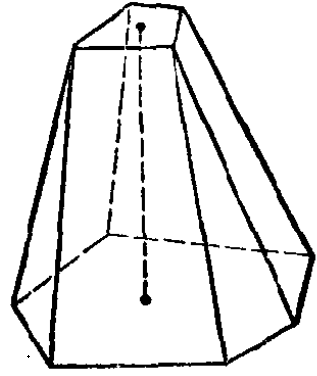
\includegraphics[width=4cm]{../pic/ltjh-ch2-68.png}
        \caption{}\label{fig:ltjh-2-68}
    \end{minipage}
    \qquad \qquad
    \begin{minipage}[b]{10cm}
        \centering
        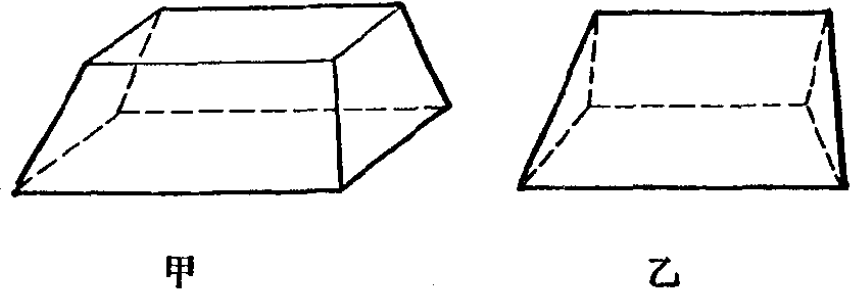
\includegraphics[width=10cm]{../pic/ltjh-ch2-69.png}
        \caption{}\label{fig:ltjh-2-69}
    \end{minipage}
\end{figure}

显然,拟柱体的侧面是三角形、梯形或平行四边形。

两底面是矩形,并且它们的对应边平行,这样的拟柱体叫做\zhongdian{长方台}(图 \ref{fig:ltjh-2-69} 甲)。
如果拟柱体的下底面是梯形或平行四边形,上底面变成了与下底面的平行边平行的线段,这样的拟柱体叫做\zhongdian{楔体}(图 \ref{fig:ltjh-2-69} 乙)。

利用棱锥体积公式,可以求出拟柱体的体积。

\begin{dingli}[定理][dl:nizhuti-tj]
    如果拟柱体的上、下底面的面积为 $\bm{S'}$、$\bm{S}$,中截面的面积为 $\bm{S_0}$,高为 $\bm{h}$,那么它的体积是
    \begin{center}
        \framebox[16em]{$\bm{V_\text{拟柱体} = \exdfrac{1}{6} h (S + 4S_0 + S')}$。}
    \end{center}
\end{dingli}

\zhengming 如图 \ref{fig:ltjh-2-70},在拟柱体 $ABCDEF{-}A'B'C'D'$ 的中截面 $A_1D_1$ 内任取一点 $P$,
并且把它和这个拟柱体的各个顶点分别连结起来。 这样,把拟柱体分成若干个以 $P$ 为顶点的棱锥,
拟柱体的体积等于这些棱锥体积的和。

我们把这些棱锥分成两类:一类是以拟柱体的底面为底的,一类是以拟柱体的侧面为底的。

第一类的棱锥有两个,棱锥 $P{-}AC$ 和棱锥 $P{-}A'C'$。 它们的体积分别是:
\begin{align*}
    & V_{P{-}AC} = \exdfrac{1}{3} S \cdot \exdfrac{1}{2} h = \exdfrac{1}{6} hS \douhao \\
    & V_{P{-}A'C'} = \exdfrac{1}{3} S' \cdot \exdfrac{1}{2} h = \exdfrac{1}{6} hS' \juhao
\end{align*}

\begin{wrapfigure}[10]{r}{5.5cm}
    \centering
    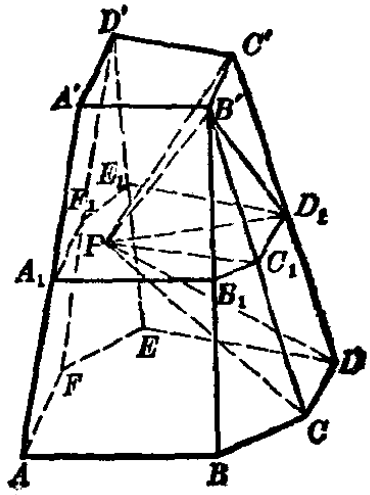
\includegraphics[width=4.5cm]{../pic/ltjh-ch2-70.png}
    \caption{}\label{fig:ltjh-2-70}
\end{wrapfigure}

在第二类棱锥中,我们先求其中的一个,例如棱锥 $P{-}CC'$ 的体积。
因为棱锥 $P{-}C_1D_1B'$ 和棱锥 $P{-}CC'$ 的底面在同一个平面上,顶点相同,所以它们的高相等。
又因为梯形 $CDC'B'$ 的面积等于 $\triangle C_1D_1B'$ 的面积的 4 倍,(为什么?)所以
$$ V_{P{-}CC'} = 4 V_{P{-}C_1D_1B'} \juhao $$

另一方面,
\begin{align*}
    V_{P{-}C_1D_1B'} &= V_{B'{-}PC_1D_1} \\
                     &= \exdfrac{1}{3} \cdot \exdfrac{h}{2} \cdot S_{\triangle PC_1D_1} \\
                     &= \exdfrac{1}{6} h S_{\triangle PC_1D_1} \douhao
\end{align*}

$\therefore$ \quad $V_{P{-}CC'} = \exdfrac{1}{6} h \cdot 4 S_{\triangle PC_1D_1}$。

同样可以证明:
\begin{align*}
    & V_{P{-}DD'} = \exdfrac{1}{6} h \cdot 4 S_{\triangle PD_1E_1} \douhao \\
    & \cdots \cdots
\end{align*}

把第二类棱锥的体积相加,得
\begin{align*}
    & \exdfrac{1}{6}h (4 S_{\triangle PC_1D_1} + 4 S_{\triangle PD_1E_1} + \cdots ) = \exdfrac{1}{6} h \cdot 4 S_0 \juhao \\
    & V_{\text{拟柱体}} = \exdfrac{1}{6} hS + \exdfrac{1}{6} h \cdot 4 S_0 + \exdfrac{1}{6} hS' = \exdfrac{1}{6} h (S + 4S_0 + S') \juhao
\end{align*}

棱柱、棱锥、棱台是特殊的拟柱体,它们的体积公式有下面的关系。

当拟柱体的上、下底面是对应边平行的全等多边形时,它就是棱柱,这时,$S' = S_0 = S$,公式变为 $V = Sh$;

当拟柱体的上底面退缩成一点时,它就是棱锥,这时,$S' = 0$,$S_0 = \exdfrac{1}{4} S$,公式变为 $V = \exdfrac{1}{3} Sh$;

当拟柱体的上、下底面是对应边平行的相似多边形时,它就是棱台。根据 \ref{subsec:2-3} 节例 2可知,$2\sqrt{S_0} = \sqrt{S} + \sqrt{S'}$,
即 $4S_0 = S + 2\sqrt{SS'} + S'$,得 $V= \exdfrac{1}{3} h (S + \sqrt{SS'} + S')$。

因此棱柱、梭锥、棱台的体积公式也都可写成
$$ V = \exdfrac{1}{6} h (S' + 4S_0 + S) \juhao $$


\liti[0] 一草垛下部是倒长方台形,上部是以长方台的上底为底的楔体形。
已知长方台上底面边长约为 8.4 m 和 4.2 m,下底面边长约为 7.6 m 和 3.0 m,高是 2.2 m。
楔体形上面的棱长约为 5.8 m,高约为 1.5 m。 求这垛草的重量约多少斤(每一立方米的草重约 300 斤)。

\begin{wrapfigure}[4]{r}{5.5cm}
    \centering
    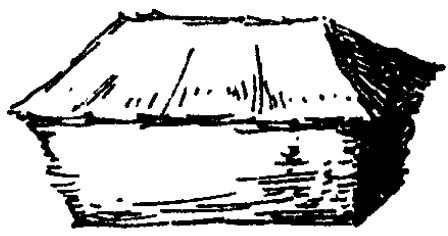
\includegraphics[width=5cm]{../pic/ltjh-ch2-71.png}
    \caption{}\label{fig:ltjh-2-71}
\end{wrapfigure}

\jie 长方台的中截面的边长分别是 $\exdfrac{1}{2} (8.4 + 7.6)$ m 和 $\exdfrac{1}{2} (4.2 + 3.0)$ m 。

$\therefore$ \quad $S_0 = \exdfrac{1}{2} (8.4 + 7.6) \times \exdfrac{1}{2} (4.2 + 3.0) \approx 28.8 \; (\pfm)$,

\qquad $\begin{aligned}
    V_\text{长方台} &= \exdfrac{1}{6} \times 2.2 \times (8.4 \times 4.2 + 4 \times 28.8 + 7.6 \times 3.0) \\
                    &\approx 63.5 \; (\lfm) \juhao
\end{aligned}$

楔体是上底面面积为零的拟柱体,它的中截面边长是 $\exdfrac{1}{2} (8.4 + 5.8)$ m 和 $\exdfrac{1}{2} \times 4.2$ m。

$\therefore$ \quad $S_0 = \exdfrac{1}{2} (8.4 + 5.8) \times \exdfrac{1}{2} \times 4.2 \approx 14.9 \; (\pfm)$,

\qquad $V_\text{楔体} = \exdfrac{1}{6} \times 1.5 \times (4 \times 14.9 + 8.4 \times 4.2) \approx 23.7 \; (\lfm)$。

草垛休积 $V = 63.5 + 23.7 \approx 87 \; (\lfm)$。

重量 $W = 300 \times 87 \approx 2.6 \times 10^4 \; (\text{斤})$。

答:这垛草重约 2.6 万斤。


\begin{lianxi}

已知拟柱体的下底面面积为 $20\;\pflm$,上底面面积为 $6\;\pflm$,
中截面面积为 $12\;\pflm$,高为 15 cm。求这个拟柱体的体积。

\end{lianxi}

\end{enhancedline}

